\documentclass[11pt,a4paper]{article}
\usepackage[margin=23mm]{geometry}
\usepackage{graphicx,booktabs,longtable,amsmath,amssymb,array}
\usepackage[T1]{fontenc}
\usepackage{lmodern}
\usepackage[hidelinks]{hyperref}
\usepackage{microtype}
\setlength{\parskip}{5pt}
\setlength{\parindent}{0pt}
\renewcommand{\thetable}{S\arabic{table}}
\renewcommand{\thefigure}{S\arabic{figure}}
\title{Supplementary Methods and Results\\\large Batch-dependent negative sampling and marginal-preserving decoy construction in TCR--peptide benchmarks}
\author{Sharon Melhi and Rajat Bhardwaj\\[3pt]
\small Amity School of Engineering and Technology,\\
\small Amity University Bengaluru, Bengaluru, India\\
\small Corresponding author: Sharon Melhi, \href{mailto:sharonmelhi365@gmail.com}{sharonmelhi365@gmail.com}}
\date{}
\begin{document}
\maketitle
\begin{center}\small Online Resource 1\\Network Modeling Analysis in Health Informatics and Bioinformatics\end{center}
\section{Data eligibility and reconstruction}
The source is the untouched VDJdb release dated 1 June 2023. The following SHA-256 strings concatenate across the displayed line break without spaces.
\begin{quote}\small
ZIP archive:\par\texttt{7c4994ce32eba8e0ff6c23d1ec53b85a982b}\\\texttt{e69651ed1f467ffe64c86c66c1d1}\par
Extracted \texttt{vdjdb.txt}:\par\texttt{2823281ece02f37b15cdd9187be374e99ee}\\\texttt{7b46e041572fc2cde4b295a9bf52e}
\end{quote}
Read the TSV with empty strings preserved and add a zero-based source-row index before filtering. Sequential row counts are in Table~\ref{tab:filters}.
\begin{table}[h]\centering
\caption{Deterministic filtering before confidence selection and tuple deduplication.}\label{tab:filters}
\begin{tabular}{lr}
\toprule
Filter retained sequentially & Rows\\
\midrule
Frozen release & 92,771\\
Human species & 85,329\\
TRB chain & 49,686\\
Class-I MHC & 47,005\\
Two-field HLA source-label syntax & 35,278\\
Canonical CDR3-beta & 35,242\\
Canonical peptide, length 8--15 & 35,237\\
\bottomrule
\end{tabular}

\end{table}
Species, gene and MHC class are exact source values \texttt{HomoSapiens}, \texttt{TRB} and \texttt{MHCI}. Full-string matching uses the following regular expressions:
\begin{verbatim}
HLA:      HLA-[ABC]\*\d{2}:\d{2}
CDR3beta: C[ACDEFGHIKLMNPQRSTVWY]*[FW]
Peptide:  [ACDEFGHIKLMNPQRSTVWY]{8,15}
\end{verbatim}
The HLA expression validates syntax only, not existence in a nomenclature dictionary. Confidence filtering precedes deduplication by beta, peptide and source HLA label, retaining the first eligible source row. The full eligible tuple set defines the all-score registry.

The primary data contain two records under unresolved \texttt{HLA-A*08:01}, neither retained by assignment, and 72 under the legacy annotation \texttt{HLA-A*24:01}, of which 26 are retained. All 41 source labels were checked against active two-field prefixes in IPD-IMGT/HLA version 3.52.0 (17 April 2023); only these two lacked a match. That frozen release's deleted-allele registry lists historical A*2401 (HLA00049) as deleted in March 1995 because its sequence contained errors. Evidence is pinned to official Git commit \texttt{38398a75e9762ff070d8e9bd714d074332646cd7} in \url{https://github.com/ANHIG/IMGTHLA}; checksums and download URLs are in \texttt{official\_annotation\_validation.json}. A matching name establishes nomenclature compatibility, not assay-annotation accuracy. The source labels are not silently recoded. Excluding both from positive cohorts and the registry leaves 3,108 primary tuples, 251 peptides and 39 source strata; assignment retains 2,665 tuples, 235 peptides and 21 strata. Its complete manifest equals the original manifest with those strata removed. The expected invariants remain exact; HLA-distribution TV between original and retained positives becomes 0.11884. A separate A*08:01-only sensitivity leaves the 2,691-row assignment entirely unchanged. ``HLA stratum'' thus means source annotation, and losing a flagged label must not be interpreted as losing a genuine allele.

The source sampler was independently rerun on both the 3,108-row full population and the 2,665-row common retained population, with 30 seeds per order. On the former, contradiction rates were 2.8882\%, 0.9331\% and 0.2445\% for release, sorted and shuffled loading; peptide total variations were 0.18294, 0.43917 and 0. The corresponding identity-oracle AUROCs were 0.64230, 0.79357 and 0.50000. Exact receptor groups and models were also rebuilt after these exclusions: peptide-plus-HLA AUROC was 0.561857 for sorted loading (all-run range 0.553202--0.573754), 0.518775 for release order (0.513858--0.523180), and 0.500000 for shuffling and assignment. The five fold seeds retained 2,618, 2,625, 2,636, 2,642 and 2,621 positives, respectively. These reproduce the qualitative construction findings after annotation exclusions. Complete per-seed values, rather than an assumption of unchanged results, accompany this sensitivity.

Antigen-donor indices in the reconstruction manifests are \emph{representative identifiers}: each selects the first source row with the required peptide--HLA value and reconstructs the decoy tuple. These identifiers do not necessarily name the donor row selected internally by the sampler and cannot certify a permutation. Separate assignment-witness files record the actual receiver-to-donor indices selected by the unmodified assignment routine. All 58 witnesses (33,839 assignments) were independently checked for equal retained receiver/donor sets, absence of fixed points, within-stratum cycles, registry exclusion and tuple agreement with the reconstruction manifests. They cover the primary and score-3 assignments, annotation sensitivity, five distance-separated tests and all 25 primary plus 25 annotation-filtered folds.

The data archive retains its source license. The reproduction package includes the original unmodified archive, aggregate measurements and zero-based receiver/donor row identifiers. Derived sequence CSV files are generated locally and excluded from distribution. A donor value of $-1$ identifies the source sampler's hard-coded \texttt{AAAAA}/\texttt{A*02:01} sentinel. An independently executed reconstruction check compared 82 manifests, representing 219,181 decoys, with the local sequence materializations and found exact equality.

\section{Audited selection logic and randomization}
The sampler class is executed directly from its Python abstract syntax tree with tagged placeholder embeddings. A minimal array shim implements the tensor operations needed to recover selected sequence identities. Embedding models, network weights and training are not part of this execution. The positive set is assigned to a class attribute but never loaded by the selection routine. The exact pinned implementation, executable audit, source provenance and unchanged license notices are supplied in the public reproducibility archive at \url{https://github.com/Sharon-codes/Precision-Oncology}, research revision \texttt{a4162ded50ba24d76ab8d5134577eba6935f910b}.

For non-singleton batches, a randomized index derangement is followed by swaps intended to repair equal-peptide matches. Rows still matching their own peptide draw from a distinct peptide--HLA pool. Up to 20 independent draws seek a different peptide before a sentinel is emitted. The fallback pool samples unique ligand values, whereas the initial permutation samples rows. Both peptide and HLA move with the donor; the receiver's original HLA is not a constraint in the source sampler. A two-receptor cross-reactivity fixture generates two registry contradictions out of two negatives with either the true or empty positive set. A one-peptide fixture uses all 20 attempts and emits the sentinel. These fixtures establish branch behavior, not public-cohort rates.

Public source-sampler seeds are 0--29. Shuffled input order uses NumPy's default random generator with seed $100000+\mathrm{seed}$; the sampler uses Python's seeded random generator. Synthetic order randomization instead uses Python's random generator with the same seed offset, as recorded in its own script, across seeds 0--99. Pool ordering remains fixed within a cohort. Main batch sizes are 16, 64 and 256; other confidence cohorts use 64. The common-population comparison holds all 2,691 retained positive tuples fixed. The full main grid contains 541 construction runs (including the deterministic assignment), generating 3,770,361 decoys. Additional rejection, fold and split analyses are recorded separately and are not counted as independent biological samples.

\section{Why independent rejection changes the marginal}
Let $E_i$ denote eligible donor rows for receptor row $i$ in its HLA stratum. Independent uniform draws from $E_i$ give donor $j$ expected weight
\begin{equation}
q_j=\frac{1}{N}\sum_{i=1}^N\frac{\mathbf{1}[j\in E_i]}{|E_i|}.
\end{equation}
This need not equal the original donor-row weight $1/N$. Summing $q_j$ across rows sharing a peptide gives its expected negative marginal. For example, peptide frequencies $(1/2,1/4,1/4)$ with each receptor excluded only from its own peptide yield expected negative peptide frequencies $(1/3,1/3,1/3)$, despite a feasible exact marginal-preserving permutation. Their total variation is $1/6$. In the actual retained cohort, expected peptide TV is 0.10199944; the mean realized TV is 0.13485693 across 30 seeds, which also includes finite sampling variation. These are distinct quantities.

\section{Assignment certificates and failure boundaries}
For each source HLA stratum, build the square matrix with admissible off-diagonal costs 0, diagonal costs 1 and forbidden costs $n+1$, and minimize full assignment cost. The all-diagonal solution supplies a feasible upper bound of $n$. Every optimal solution therefore avoids forbidden edges. Removing fixed points leaves a union of closed permutation cycles and maximizes retained rows because the objective equals the number discarded. A generic maximum bipartite matching does not enforce closure: a three-node directed path has matching size two and closed retention zero. The method's optimality statement applies only to this explicitly defined contract.

Every output is checked for: equal positive and negative counts; no tuple in the reference registry; a common retained source/donor row set; unchanged receiver HLA; and exact receptor, peptide, HLA and joint peptide--HLA marginal equality. A separate exhaustive verifier compared the implementation against all permutations on 166 fixtures, examining 924,960 permutations. Fixtures included 130 with repeated beta identities, 136 with repeated peptide identities and 38 with multiple HLA strata. All checks passed. Additional reviewers independently tested random small instances. These tests support combinatorial correctness, not biological validity or large-scale runtime.

Within any stratum, a peptide occupying more than half the rows precludes a full different-peptide permutation. More complicated registered cross-reactivity can also prevent full retention. The score-3 cohort contains a global majority peptide at 186/320, so failure is already inevitable even without HLA constraints. Repeated beta or peptide values can generate identical negative triples from distinct row assignments; the main assignment includes 67 duplicate negative rows. Alternative optimum cycles are not claimed equivalent biologically.

\section{Peptide-distance construction sensitivity}
All pairwise unit-cost Levenshtein distances were calculated for the 253 main-cohort peptides. Joining pairs at distance at most two produced 221 connected components. For split seeds 0--4, component identifiers were permuted using \texttt{default\_rng(200000+seed)}, then the first 132, next 44 and final 45 assigned to training, validation and test. Component counts, rather than record counts, set the nominal proportions. All five partitions had minimum cross-partition distance 3. Source candidate pools and corrected donor rows stayed inside the relevant test partition; the external registry was only an exclusion reference.
\begin{table}[h]\centering\small
\caption{Distance-separated partition sizes and test retention. No predictive model was fitted in this analysis.}\label{tab:splits}
\begin{tabular}{lrrrrr}
\toprule
Seed & Train & Validation & Test & Retained test & Retained (\%)\\
\midrule
0 & 1629 & 531 & 1022 & 509 & 49.80\\
1 & 1771 & 534 & 877 & 546 & 62.26\\
2 & 1808 & 731 & 643 & 380 & 59.10\\
3 & 1703 & 1107 & 372 & 271 & 72.85\\
4 & 2153 & 436 & 593 & 190 & 32.04\\
\bottomrule
\end{tabular}

\end{table}
The source sampler was run ten times per order on each full test population and each common retained population. Deterministic assignments were also evaluated, producing 305 construction records in total. Every corrected test population had zero registry contradictions and exact declared marginals. Their coverage ranged from 32.04\% to 72.85\%, underscoring that construction certificates and biological coverage are separate outcomes.

\section{Trained controls and placement sensitivity}
Exact receptor groups were sorted, shuffled by each fold seed (17, 41, 73, 107, 211) and divided into five group blocks. In the primary protocol each fold is independently matched before compared samplers construct decoys on its retained positives. Negative random seeds are \texttt{sampling\_seed + 10000 * fold}, for sampling seeds 0--9. Groups never cross folds. The same retained positive multiset is asserted for each comparator within a fold seed, although changing the fold seed changes feasible retention.

For each held-out fold, one-hot encoders are fitted only on the other folds and unseen categories are ignored. L2 logistic regression uses $C=1$, \texttt{liblinear}, tolerance $10^{-8}$, maximum 2,000 iterations and random state 1729, without test-set tuning. Four feature sets are evaluated: peptide identity; HLA identity; concatenated peptide and HLA identities; receptor identity. Training folds are balanced by class; AUROC is calculated from the complete pooled out-of-fold score vector. Per-fold metrics and unseen-category proportions are retained. Receptor-only outputs equal 0.5; an archived synthetic positive control with 100 artificial receptor groups and 200 pairs, evaluated under two fold seeds through the same fitting pipeline, returns peptide and peptide-plus-HLA AUROC 1.0 and HLA/receptor-only AUROC 0.5. Its 400 out-of-fold prediction rows, eight pooled metrics and 40 fold metrics are supplied. Models therefore distinguish positive controls from structural nulls.

Table~\ref{tab:trained} supplies complementary metrics for the peptide-plus-HLA model. Average precision (AP) and Brier values describe the balanced synthetic-decoy task, not prevalence-calibrated clinical performance. Mean unseen test-peptide category fractions in the split-first protocol were 4.08\% (assignment), 4.88\% (sorted), 4.34\% (release order) and 4.08\% (shuffled). Such categories were retained in scoring.
\begin{table}[h]\centering\small
\caption{Trained peptide-plus-HLA control means. AP is average precision. Each source value averages five fold assignments and ten decoy seeds. Matching averages the five deterministic fold assignments; its global construction is fixed.}\label{tab:trained}
\begin{tabular}{llrrr}
\toprule
Protocol & Sampler & AUROC & AP & Brier\\
\midrule
Split first & Release & 0.5168 & 0.5151 & 0.2497\\
Split first & Sorted & 0.5558 & 0.5548 & 0.2467\\
Split first & Shuffled & 0.5000 & 0.5000 & 0.2500\\
Split first & Assignment & 0.5000 & 0.5000 & 0.2500\\
Construct first & Release & 0.5109 & 0.5270 & 0.2569\\
Construct first & Sorted & 0.7146 & 0.7280 & 0.2106\\
Construct first & Shuffled & 0.3298 & 0.3903 & 0.2647\\
Construct first & Assignment & 0.3262 & 0.3892 & 0.2648\\
\bottomrule
\end{tabular}

\end{table}
The first global-construction experiment is retained as a sensitivity, including below-chance results. A globally balanced category satisfies $\Delta_{\rm test}=-\Delta_{\rm train}$ after a complementary split; its training label frequency can be oppositely associated with held-out frequency. This is a finite-dataset coupling mechanism, not molecular reverse recognition. Protocol placement also changes feasible retention and batch composition, so the two experiments are not a pure single-factor intervention. No score sign was selected using test outcomes.

\section{Additional cohort and batch summaries}
\begin{table}[h]\centering\scriptsize
\caption{Full-cohort sensitivity at batch size 64, before assignment exclusions. Entries are means $\pm$ sample standard deviations over 30 construction seeds. All oracle values are same-dataset marginal diagnostics.}\label{tab:confidence}
\begin{tabular}{llrrr}
\toprule
Score & Order & Contradictions (\%) & Peptide TV & Oracle AUROC\\
\midrule
$\geq0$ & Release & $6.8047\pm0.0479$ & $0.3904\pm0.0006$ & $0.7646\pm0.0003$\\
$\geq0$ & Sorted & $0.2052\pm0.0111$ & $0.7735\pm0.0010$ & $0.9484\pm0.0003$\\
$\geq0$ & Shuffled & $5.1545\pm0.0748$ & $0.0085\pm0.0013$ & $0.5066\pm0.0010$\\
$\geq1$ & Release & $2.9887\pm0.1022$ & $0.1294\pm0.0011$ & $0.6048\pm0.0007$\\
$\geq1$ & Sorted & $0.8820\pm0.0761$ & $0.4342\pm0.0028$ & $0.7916\pm0.0019$\\
$\geq1$ & Shuffled & $0.2284\pm0.0695$ & $0.0000\pm0.0000$ & $0.5000\pm0.0000$\\
$=3$ & Release & $1.3854\pm0.2923$ & $0.5188\pm0.0000$ & $0.8209\pm0.0041$\\
$=3$ & Sorted & $1.0417\pm0.3317$ & $0.4688\pm0.0000$ & $0.7910\pm0.0024$\\
$=3$ & Shuffled & $0.0938\pm0.1672$ & $0.1671\pm0.0077$ & $0.6069\pm0.0050$\\
\bottomrule
\end{tabular}

\end{table}
\begin{figure}[h]\centering
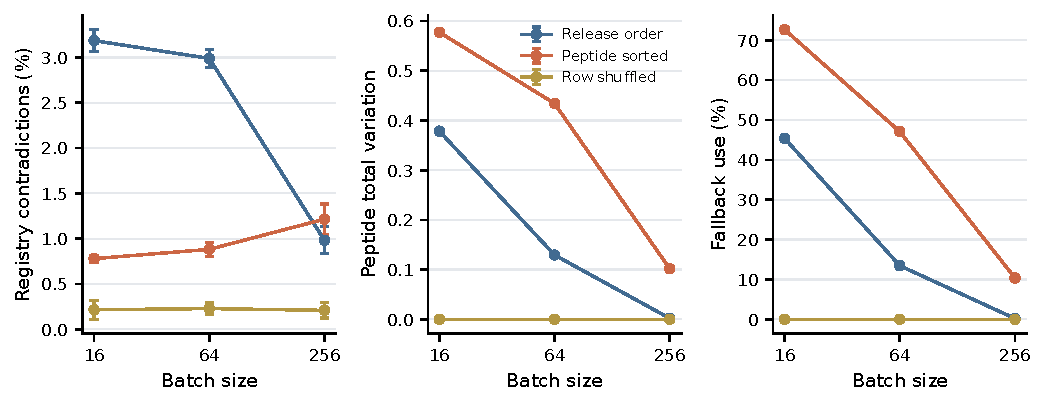
\includegraphics[width=\textwidth]{figures/FigS1.pdf}
\caption{Batch-size sensitivity on the complete primary cohort. Points and error bars are sampler-seed means and standard deviations. Lines connect the three tested conditions for readability and do not represent fitted models. Shuffled peptide TV was zero in all main-cohort runs; registry contradictions persisted.}
\end{figure}
\clearpage
\begin{longtable}{lrrrr}
\caption{Complete retention by source HLA annotation stratum. Flagged labels A*08:01 and A*24:01 are discussed in Supplementary Methods.}\label{tab:fullhla}\\
\toprule
Source label & Original & Retained & Peptides & Retained (\%)\\
\midrule\endfirsthead
\toprule Source label & Original & Retained & Peptides & Retained (\%)\\\midrule\endhead
HLA-A\textasteriskcentered{}01:01 & 172 & 82 & 10 & 47.7\\
HLA-A\textasteriskcentered{}02:01 & 1367 & 1367 & 106 & 100.0\\
HLA-A\textasteriskcentered{}02:06 & 2 & 0 & 1 & 0.0\\
HLA-A\textasteriskcentered{}03:01 & 71 & 71 & 15 & 100.0\\
HLA-A\textasteriskcentered{}08:01 & 2 & 0 & 1 & 0.0\\
HLA-A\textasteriskcentered{}11:01 & 161 & 161 & 9 & 100.0\\
HLA-A\textasteriskcentered{}24:01 & 72 & 26 & 2 & 36.1\\
HLA-A\textasteriskcentered{}24:02 & 77 & 61 & 14 & 79.2\\
HLA-A\textasteriskcentered{}25:01 & 1 & 0 & 1 & 0.0\\
HLA-A\textasteriskcentered{}29:02 & 3 & 3 & 3 & 100.0\\
HLA-A\textasteriskcentered{}30:02 & 6 & 4 & 2 & 66.7\\
HLA-A\textasteriskcentered{}32:01 & 1 & 0 & 1 & 0.0\\
HLA-A\textasteriskcentered{}68:01 & 31 & 8 & 3 & 25.8\\
HLA-B\textasteriskcentered{}07:02 & 328 & 328 & 22 & 100.0\\
HLA-B\textasteriskcentered{}08:01 & 228 & 146 & 10 & 64.0\\
HLA-B\textasteriskcentered{}14:02 & 1 & 0 & 1 & 0.0\\
HLA-B\textasteriskcentered{}15:01 & 2 & 2 & 2 & 100.0\\
HLA-B\textasteriskcentered{}18:01 & 2 & 2 & 2 & 100.0\\
HLA-B\textasteriskcentered{}27:05 & 130 & 38 & 2 & 29.2\\
HLA-B\textasteriskcentered{}35:01 & 109 & 109 & 5 & 100.0\\
HLA-B\textasteriskcentered{}35:08 & 34 & 34 & 12 & 100.0\\
HLA-B\textasteriskcentered{}38:01 & 3 & 3 & 3 & 100.0\\
HLA-B\textasteriskcentered{}40:01 & 2 & 2 & 2 & 100.0\\
HLA-B\textasteriskcentered{}42:01 & 140 & 140 & 7 & 100.0\\
HLA-B\textasteriskcentered{}44:02 & 2 & 0 & 1 & 0.0\\
HLA-B\textasteriskcentered{}44:03 & 2 & 0 & 1 & 0.0\\
HLA-B\textasteriskcentered{}44:05 & 1 & 0 & 1 & 0.0\\
HLA-B\textasteriskcentered{}51:01 & 13 & 0 & 1 & 0.0\\
HLA-B\textasteriskcentered{}57:01 & 145 & 80 & 6 & 55.2\\
HLA-B\textasteriskcentered{}57:06 & 1 & 0 & 1 & 0.0\\
HLA-B\textasteriskcentered{}81:01 & 16 & 0 & 1 & 0.0\\
HLA-C\textasteriskcentered{}01:02 & 2 & 0 & 1 & 0.0\\
HLA-C\textasteriskcentered{}03:03 & 1 & 0 & 1 & 0.0\\
HLA-C\textasteriskcentered{}03:04 & 1 & 0 & 1 & 0.0\\
HLA-C\textasteriskcentered{}04:01 & 1 & 0 & 1 & 0.0\\
HLA-C\textasteriskcentered{}05:01 & 1 & 0 & 1 & 0.0\\
HLA-C\textasteriskcentered{}06:02 & 1 & 0 & 1 & 0.0\\
HLA-C\textasteriskcentered{}07:01 & 1 & 0 & 1 & 0.0\\
HLA-C\textasteriskcentered{}07:02 & 41 & 20 & 2 & 48.8\\
HLA-C\textasteriskcentered{}08:02 & 7 & 4 & 3 & 57.1\\
HLA-C\textasteriskcentered{}14:02 & 1 & 0 & 1 & 0.0\\
\bottomrule
\end{longtable}

\section{Reproducibility and limits of verification}
The supplied programs regenerate constructions, rerun metadata models, audit manifests and draw figures from stored measurements. The environment used Python 3.12.14, NumPy 2.3.5, pandas 2.2.3 and SciPy 1.17.0; the exact scikit-learn and Matplotlib versions are pinned in the package. Source-row manifests, not modified biological sequence tables, are the redistribution interface. Software versions and row order are relevant to exact assignments when several optima exist.

The main study is an exploratory computational audit. There was no prospective protocol registration and no original neural checkpoint evaluation. Seed variation is conditional on the fixed source release, and no biological population confidence interval or acceptance guarantee is claimed. Source annotation errors, incomplete binding ascertainment, omitted receptor context and reduced HLA/peptide coverage limit biological interpretation even when all computational assertions pass.
\section{Additional implementation considerations}
Several limits constrain interpretation. The empirical source audit concerns one implementation and one dated database release; it does not establish the prevalence of the defect across unrelated published methods. The public cohort was assembled for this audit and does not reconstruct unavailable cohorts or learned checkpoints. Registry-based sanitation is retrospective and depends on evidence quality, database completeness and the chosen beta-level key. No generated decoy has been experimentally confirmed as a nonbinder. No affinity, contact map, clinical specificity or prospective precision was measured. Equal marginal distributions also leave other shortcuts and interaction-dependent artefacts uncontrolled.

Assignment is deterministic for the specified data order and software environment. Alternative optimal cycles can change individual decoys while preserving the certified invariants; their biological consequences remain untested. Repeated identities produce duplicate negative tuples, and omission of infeasible strata changes the population. Dense assignment may be unsuitable for very large HLA groups without a sparse or approximate implementation. The trained controls use simple antigen metadata, not an interaction-aware receptor model. Such models and independent assay-confirmed nonbinders would be required to evaluate whether the construction changes biological generalization. These limitations define the next experiments; they are not repaired by larger numbers of sampler seeds.

\end{document}
